%%%%%%%%%%%%%%%%%%%%%%% file template.tex %%%%%%%%%%%%%%%%%%%%%%%%%
%
% This is a general template file for the LaTeX package SVJour3
% for Springer journals.          Springer Heidelberg 2010/09/16
%
% Copy it to a new file with a new name and use it as the basis
% for your article. Delete % signs as needed.
%
% This template includes a few options for different layouts and
% content for various journals. Please consult a previous issue of
% your journal as needed.
%
%%%%%%%%%%%%%%%%%%%%%%%%%%%%%%%%%%%%%%%%%%%%%%%%%%%%%%%%%%%%%%%%%%%
%
% First comes an example EPS file -- just ignore it and
% proceed on the \documentclass line
% your LaTeX will extract the file if required
%\begin{filecontents*}{example.eps}
%%!PS-Adobe-3.0 EPSF-3.0
%%%BoundingBox: 19 19 221 221
%%%CreationDate: Mon Sep 29 1997
%%%Creator: programmed by hand (JK)
%%%EndComments
%gsave
%newpath
  %20 20 moveto
  %20 220 lineto
  %220 220 lineto
  %220 20 lineto
%closepath
%2 setlinewidth
%gsave
  %.4 setgray fill
%grestore
%stroke
%grestore
%\end{filecontents*}
%
\RequirePackage{fix-cm}
%
%\documentclass{svjour3}                     % onecolumn (standard format)
%\documentclass[smallcondensed]{svjour3}     % onecolumn (ditto)
%\documentclass[smallextended]{svjour3}       % onecolumn (second format)
\documentclass[twocolumn]{svjour3}          % twocolumn
%
\smartqed  % flush right qed marks, e.g. at end of proof
%
\usepackage{graphicx}
%
% \usepackage{mathptmx}      % use Times fonts if available on your TeX system
%
% insert here the call for the packages your document requires
%\usepackage{latexsym}
\usepackage{booktabs}

%requested for editor please remove before print
\usepackage{lineno}
%\linenumbers
\usepackage[round]{natbib}
%
% please place your own definitions here and don't use \def but
% \newcommand{}{}
%
% Insert the name of "your journal" with
% \journalname{myjournal}
%
\begin{document}

\title{Approaching Preplanetary Streaming Instabilities in Laboratory Experiments}
%\subtitle{Do you have a subtitle?\\ If so, write it here}

\titlerunning{Motion of Dust in Dense Clouds}        % if too long for running head

\author{Niclas Schneider$^1$, Gerhard Wurm$^1$, Jens Teiser$^1$, Hubert Klahr$^2$}

%\authorrunning{Short form of author list} % if too long for running head

\institute{$^1$             University of Duisburg-Essen, Lotharstr. 1-21, 47057 Duisburg, Germany\\
              Tel.: +49-(0)203-379-1641\\
              Fax: +49-(0)203-379-1965\\
              \email{someone@uni-due.de} \\                   %  \\
%             \emph{Present address:} of F. Author  %  if needed
           \and
        $^2$   the Heidelburger
}

\date{Received: date / Accepted: date}
% The correct dates will be entered by the editor


\maketitle

\begin{abstract}

Streaming instabilities are an important particle concentration mechanism in
protoplanetary disks but the idea is essentially only based on numerical calculations.
We carried out first laboratory experiments to approach this by laboratory studies. We observed a particle cloud trapped in
a rotating system under Earth's gravity. The experiment Stokes number is 0.0024. For average dust-to-gas ratios up to 0.02 particles behave like individual
test particles. The sedimentation speed is identical to a free falling particle.  
However, for increasing dust-to-gas ratios the motion of particles is 
increasingly sensitive to clumping. This suggests a self-amplification of a denser region 
and provides experimental evidence in supporting the concept of streaming instabilities.

\keywords{}
% \PACS{PACS code1 \and PACS code2 \and more}
% \subclass{MSC code1 \and MSC code2 \and more}
\end{abstract}


\section{Introduction}

This work is motivated by the streaming instability proposed to work in protoplanetary disks (Referenzen). Numerical simulations show that at high mass loading and gas-grain coupling times comparable to the orbital timescales overdense regions can form.
(das geht sicher besser, nur ein Platzhalter, feel free to edit and add;) 

...

Some more words on planetesimal formation.

...

The scenario of streaming instabilities is widely accepted as standard way to connect to and take over from the precluding collisional growth phases of pebbles. However, laboratory experiments are essentially missing. Holly Capelo et al. xxx considered the sedimentation of a dense cloud of particles. They report the onset of the formation of 
particle clumps. No other experimental approaches with respect to streaming are known to the authors. 
Nevertheless, having a complex two fluid (particles and gas) problem it might be worth
verifying in an experiment how particle clouds really react if the particle-to-gas mass ratio is changing in a cloud of grains that continually has to adapt to a changing gas motion.

The closest experimental setup to mimic the conditions in a protoplanetary disk is
a rotating cylindrical experiment with a cloud of particles and gas within.
Such an experiment has been used before by Blum xxx and Poppe and Blum xxx for 
aggregation studies. The setup is inspired by the idea of particle trapping in convective eddies as studied by Klahr and Henning xxx. Details are given in the experiment section.


In a simplified way, the situtation that can be studied is as follows.
A larger grain takes longer to couple to a gas flow than a smaller grain and 
sediments faster than the small grain.
But how many small particles have to be how close to each other to act like a larger grain?
And how does increasing density and closeness of grains influence the result of particle motion in a rotating system?

\section{Grain-Gas Interaction}

The motion of a single particle embedded in a gas is depending on the
gas-grain coupling time or friction time $\tau_f$. 

%It can be defined as

%\begin{equation}
%\tau_f = \frac{m}{F} \cdot v = a \cdot v
%\end{equation}

%where $F$ is the drag force acting on the particle of mass $m$ which moves relative to the gas with a speed $v$. The force accelerates the particle with acceleration $a$. 

$\tau_f$ is only well defined (constant) in flows where the drag force is proportional to gas speed. This is valid for small Reynolds numbers, which is the case here. In detail the coupling time depends on the flow regime which can be described by the Knudsen number $Kn$.
The Knudsen number is defined by the ratio between the mean free pathlength between the molecules $\lambda$ and the particle radius $r$ as

\begin{equation}
Kn = \frac{\lambda}{r}
\label{tau_no}
\end{equation}

For small $Kn$ the flow is continuous. For large $Kn$ the flow is molecular.
For molecular flow the coupling time for a spherical particle of radius $r$ is given as
\begin{equation}
\tau_{f_E} = \frac{4}{3} \frac{\rho_p}{\rho_g} \frac{r}{v_g}
\label{tau0}
\end{equation}
with $\rho_g$ as gas density, $\rho_p$ as particle density and $v_g$ as thermal gas velocity. 
For small $Kn$ Stokes law applies and it is
\begin{equation}
\tau_{f_S} = \frac{2 r^2 \rho_p}{9 \eta} 
\label{tauS}
\end{equation}
For $Kn \sim 1$ eq. \ref{tauS} can be used but adding a correction factor $f_c$.
\begin{equation}
\tau_f = \tau_{f_S} \cdot f_c
\label{tau}
\end{equation}
with $f_c$ as Cunningham correction (Referenz)
\begin{equation}
f_c = 1+Kn(1.257+0.4e^{-0.55 Kn})
\end{equation}

%$f_c$ for very large Kn is 1 and this mirrors the Stokes drag law.

If a particle is dragged through a fluid with constant external force $F_{ext}$ it will be accelerated until the drag compensates for this force.
This leads to a constant velocity $v_{rel}$ relative to the gas then. In the case of gravity with gravitational acceleration $g$ this is

\begin{equation}
v_{rel} = g \cdot \tau_f
\label{vrel}
\end{equation}

However, if the gas motion changes on a timescale $\tau_{gas}$ comparable to the friction time, this simplification no longer holds. An important quantity to describe the system therefore is the Stokes number as ratio between coupling time and typical time for gas motion variation.

\begin{equation}
St = \frac{\tau_f}{\tau_{gas}}
\end{equation}

In our case we take $\tau_{gas}$ as the rotational timescale $1/f$ of the experiment chamber as the gas follows this motion. Here, $f$ is the rotation frequency
and $St = \tau_f \cdot f$. Eq. \ref{vrel} holds for small Stokes numbers. From work on
streaming instabilities, important
changes are expected to start for  $St \geq 0.001$ to occur (Zitate).

%By adjusting the ambient gas pressure in the experiment chamber and the rotation frequency and by chosing grains of certain size and density we can vary the Stokes number within the experiment in principle.

Another important parameter is the average ratio $\epsilon$ between particle mass density and gas density $\rho_g$.

\begin{equation}
\epsilon = \frac{\frac{N \cdot m_p}{V}}{\rho_g} = \frac{4}{3} \pi r^3 \frac{N}{V} \frac{\rho_p}{\rho_g}
\end{equation}
 
Here, $\rho_p$ is the bulk density of the grains (not average solid density), $V$ is the total volume covered by particles, $N$ the total number of particles injected and $m_p$ is the grain mass.
Local motion of particle will depend on other particles as they backreact on the gas. 
%We define $\epsilon$ as average dust to gas ratio.
Grains can be considered as "test" particle if $\epsilon << 1$. 
Collective motion on simple inertia argument sets in at least if epsilon $\geq$ 1.
It is one motivation of our work to study at what point there is a density dependence of particle motion while $\epsilon$ is still well below 1.

In detail the local particle (or ''dust'') density will differ from the average value and  change the motion of local grains. In that case density is not enough as parameter. Even if local density is considered it would be important how large the local bubble would be. I.e. many particles at larger distances might have similar influence as
few particles in closer neighborhood. This complicates the situation as spatial regional limits are not well defined in a fluctuating density field. We therefore define the new parameter closeness $C_i$ of particle $i$ as

\begin{equation}
C_i = \sum_{n=1}^N \frac{1}{r_n-r_i}
\end{equation}

This includes particle number but also distances.
A graphical representation of the concept of closness is seen in fig. \ref{fig.closing}.
\begin{figure}[h]
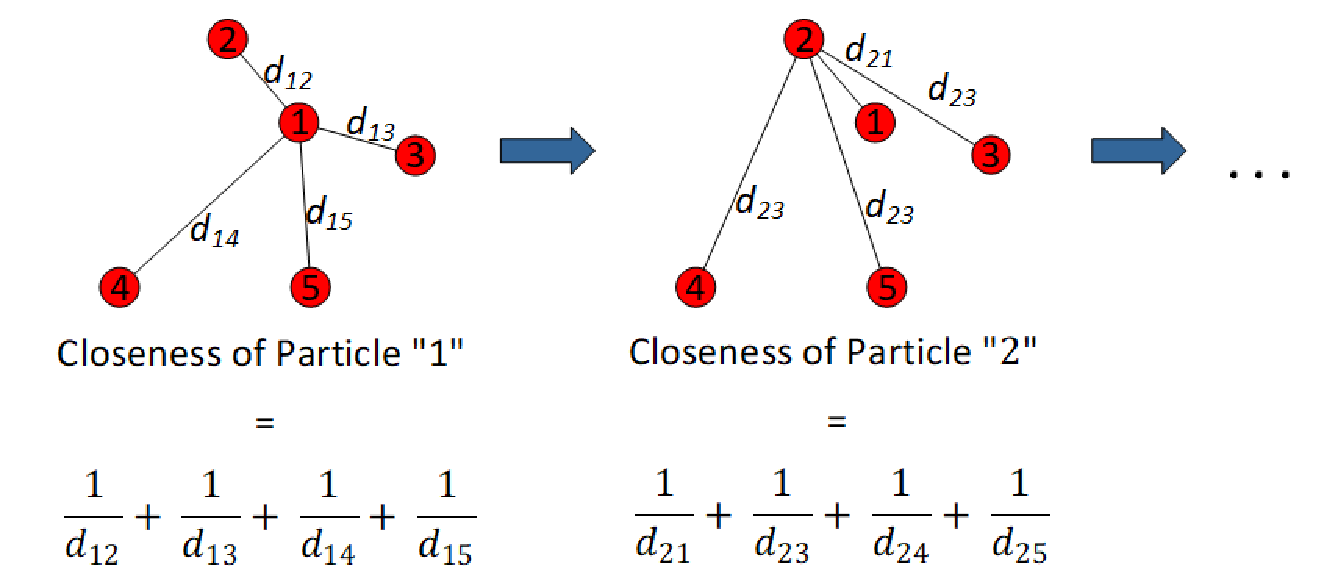
\includegraphics[width=\columnwidth]{closing.png}
    \caption{\label{fig.closing}On the definition of closeness}
\end{figure}

Closeness is often used in the literature where networks are considered (Zitate).
It might be debated, if the $1/r$-dependence in this definition is the most appropriate.
It did not enter this paper but we also tried higher orders for the analyis given below. The results were less convincing. So for this first study we
consider this definition of closeness as suitable parameter to quantify the influence of a region on an individual grain motion.

%Closeness, in general, might not be very intuitive though as a
%Having defined a closeness allows us to give a characteristic size
%of the active region as reciproke closeness.

%\begin{equation}
%R_i = \frac{1}{C_i}
%\end{equation}

Be aware that closeness is constructed from distances \textbf{and} number
of particles.
 
\section{Experiments}
\subsection{Setup}

The basic principle of the experiment used here is to prevent particles from sedimentating to the ground by trapping them in circular orbits within an eddy. This idea was proposed by
Klahr and Henning in 1997 for protoplanetary disks (fig. \ref{fig.eddy}). The same idea applies in our experiment. The only difference is that the rotation of the gas is not
induced by natural convection but rotation of an experiment chamber to which the gas
resoponds by rotating in the same way.

 
\begin{figure}[h]
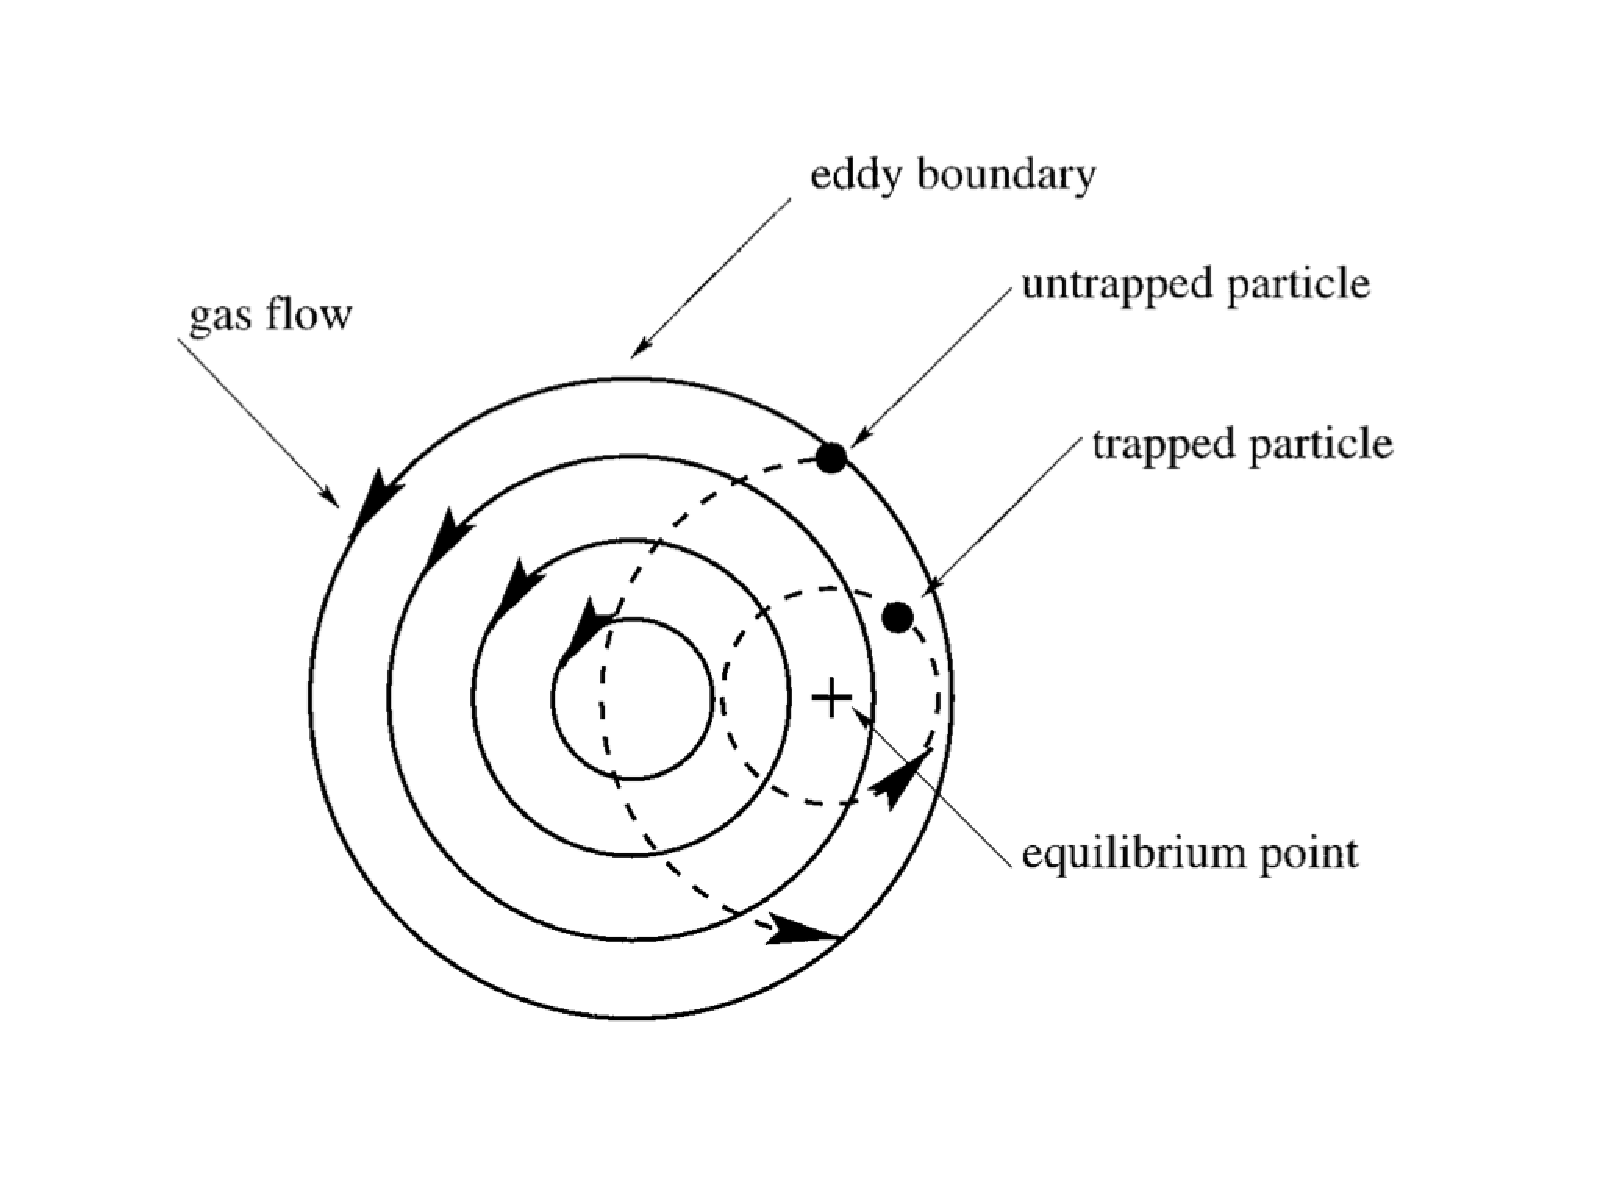
\includegraphics[width=\columnwidth]{eddy.png}
    \caption{\label{fig.eddy} Principle of particle trapping against gravity in a convective eddy of a protoplanetary disk (Klahr and Henning 1997xxx). }
\end{figure}

A sketch of the experiment can be seen in fig. \ref{fig.setup}.

\begin{figure}[h]
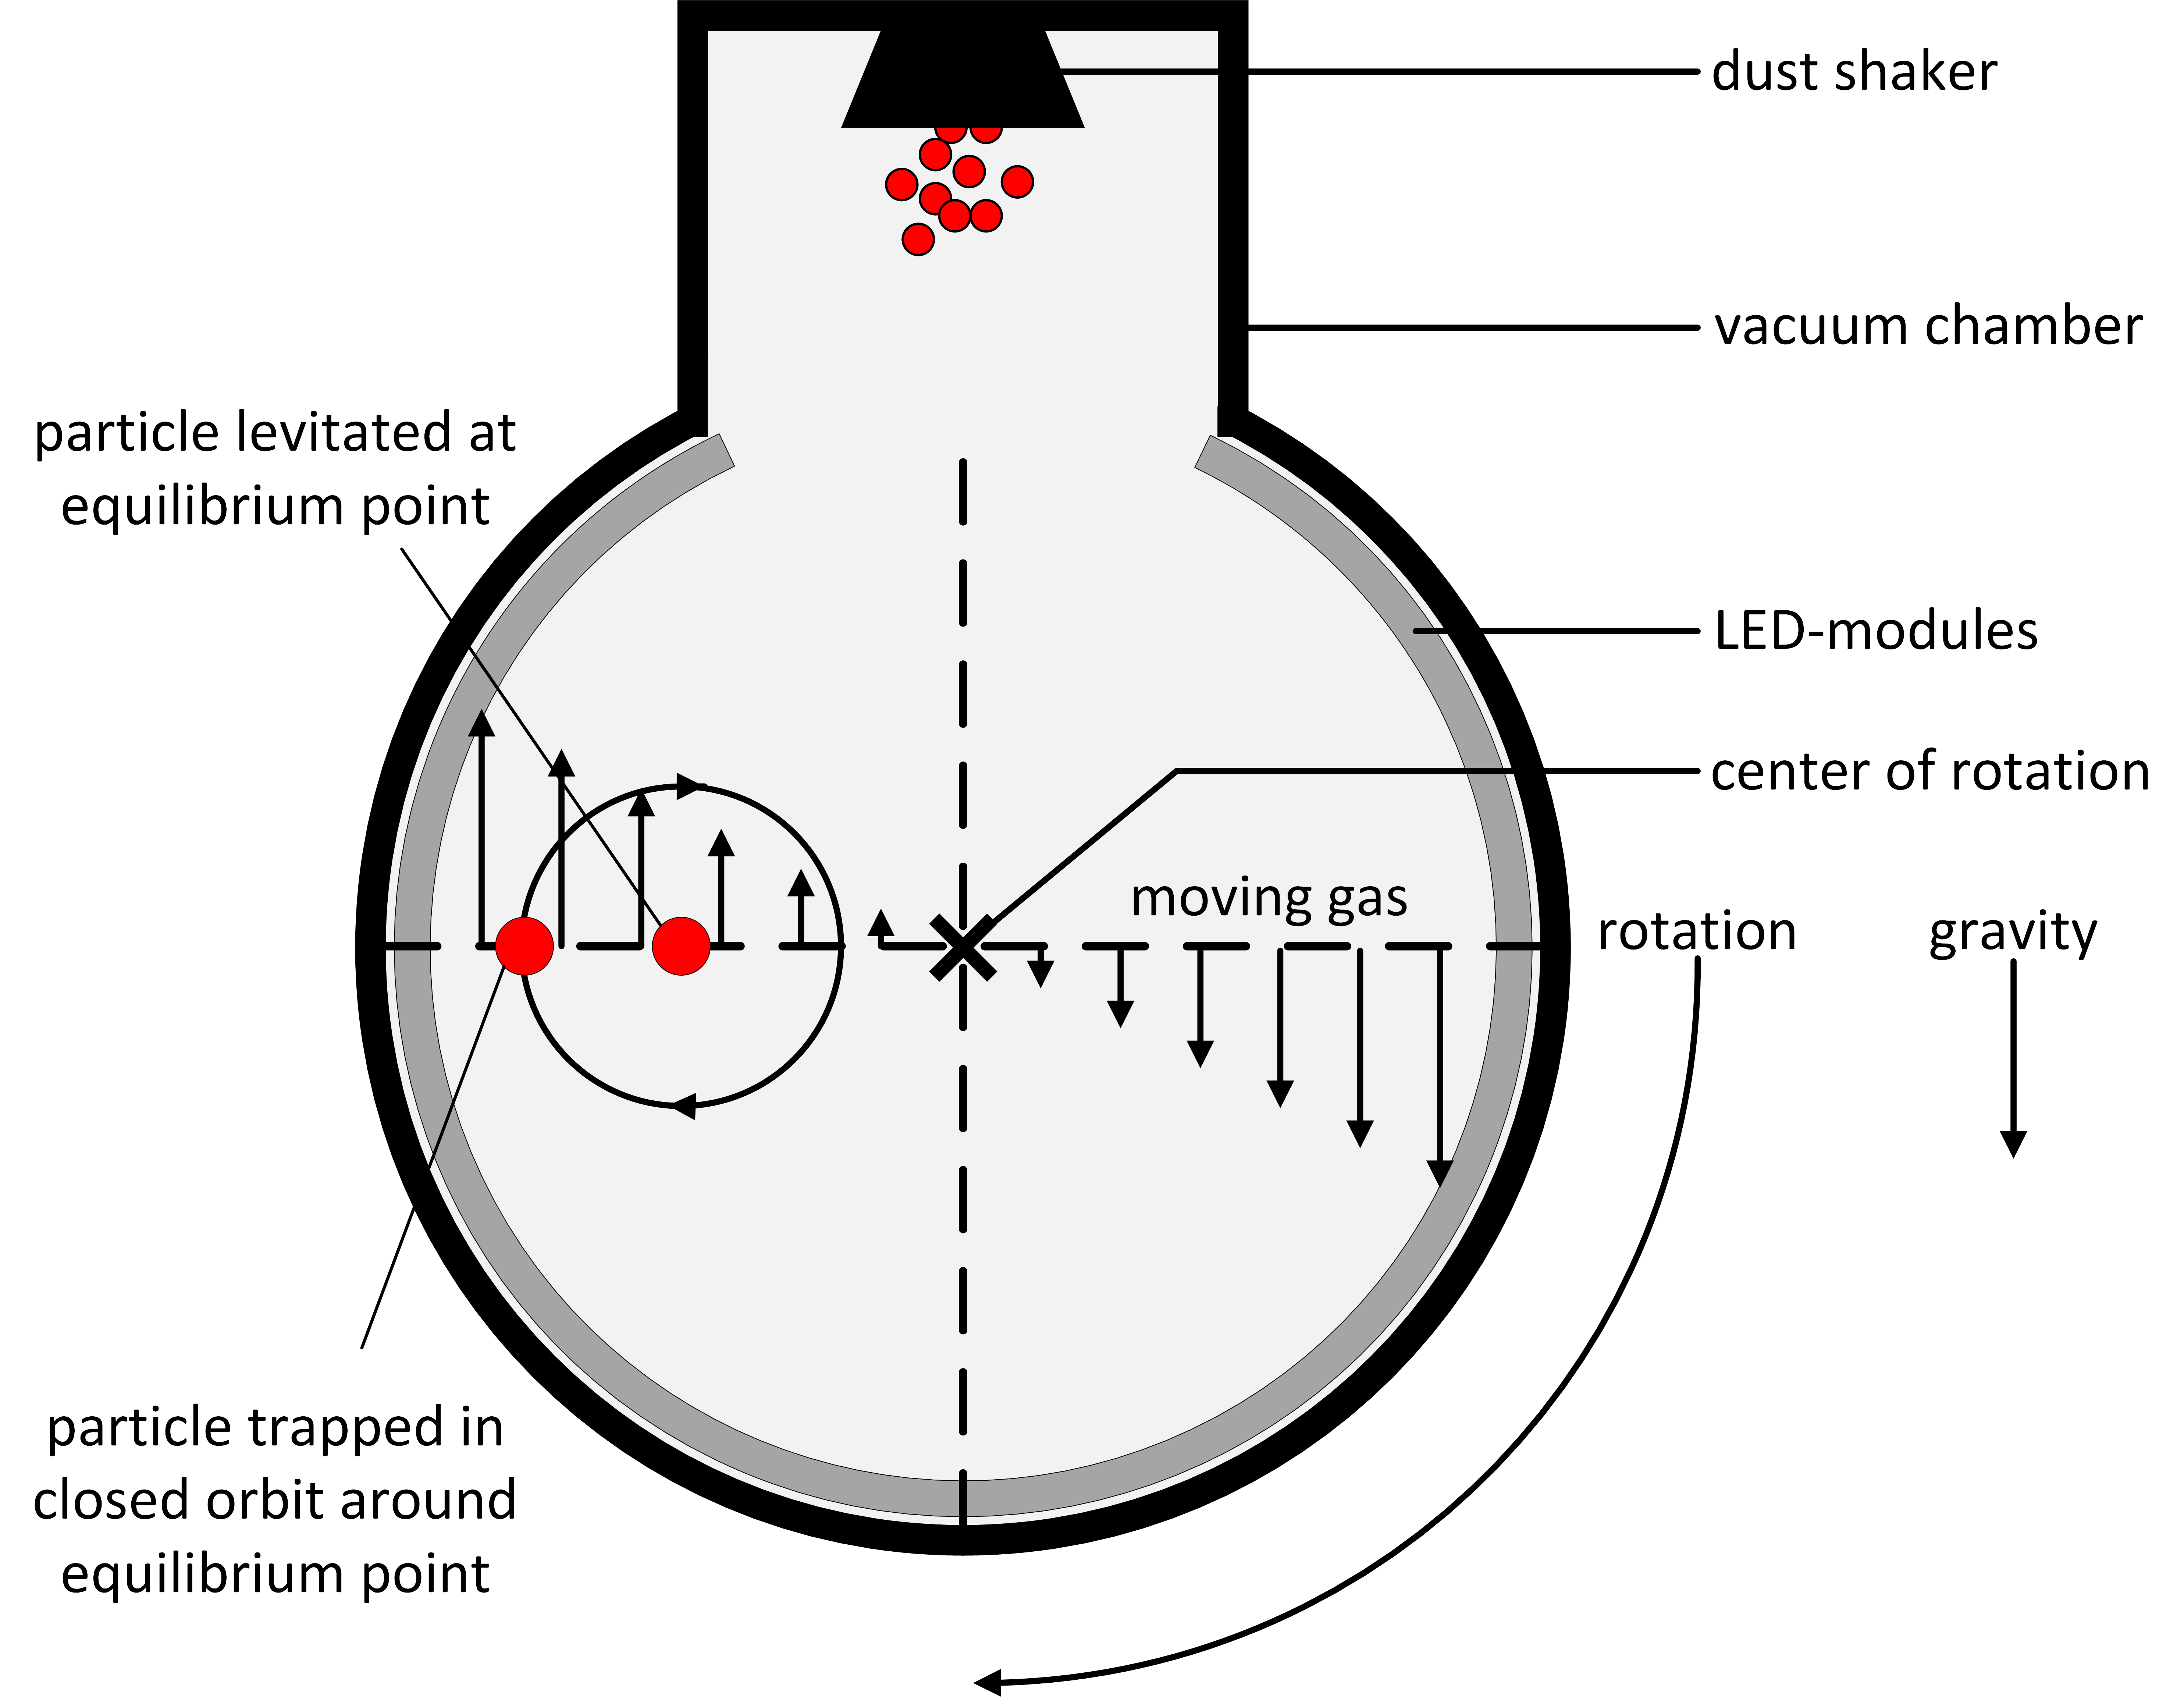
\includegraphics[width=\columnwidth]{setup.png}
    \caption{\label{fig.setup} Schematics of the experiment. Not shown are auxiliary parts. The experiment chamber is a vacuum chamber evacuated prior to experiments to a preset pressure. A camera is observing particles from the front by scattered light.}
\end{figure}

The experiment chamber is about 22 cm in diameter and is evacuated to a preset pressure before the experiment. The vacuum pump is then disconnected.
A number of electrical contacts are fed through to the rotating system. Inside the chamber a ring of LEDs generates light that
is scattered from the particles which are imaged by a camera in the front.
The particles are sieved into the chamber through a vibrating sieve, included in
an extension of the vacuum chamber. This beam of particles has a width of 5 cm and 
a thickness of 5 mm. Particles are injected while the experiment is still at rest to fill the
regions that are stable once the rotation is started. After the onset of rotation the
injection mechanism is stopped.

Real particle tracks can be seen below in fig. \ref{fig.circles}.

For the analysis, individual grain positions and tracks are generated using ImageJ (Zitat).
This makes it straight forward to determine velocities from short parts of the tracks.
With the known center of rotation of the chamber and assumed rigid rotation of the gas
the sedimentation velocity relative to the rigid gas is deduced.

\subsection{Experimental parameters}


A summary of the most important parameters of the experiment analyzed here are given in table \ref{para}.
For this first study we used hollow glass spheres to get clouds of large non-sticky particles with low density for short gas-grain coupling times. An image of the particles can be seen in
fig. \ref{fig.hollow}. While the grains have an average diameter of 165 $\rm \mu m$ and are rather sand size than dust size we will stick to terms like dust-to-gas ratio here for the relation between particle mass and gas mass. As gas we used air.

\begin{figure}[h]
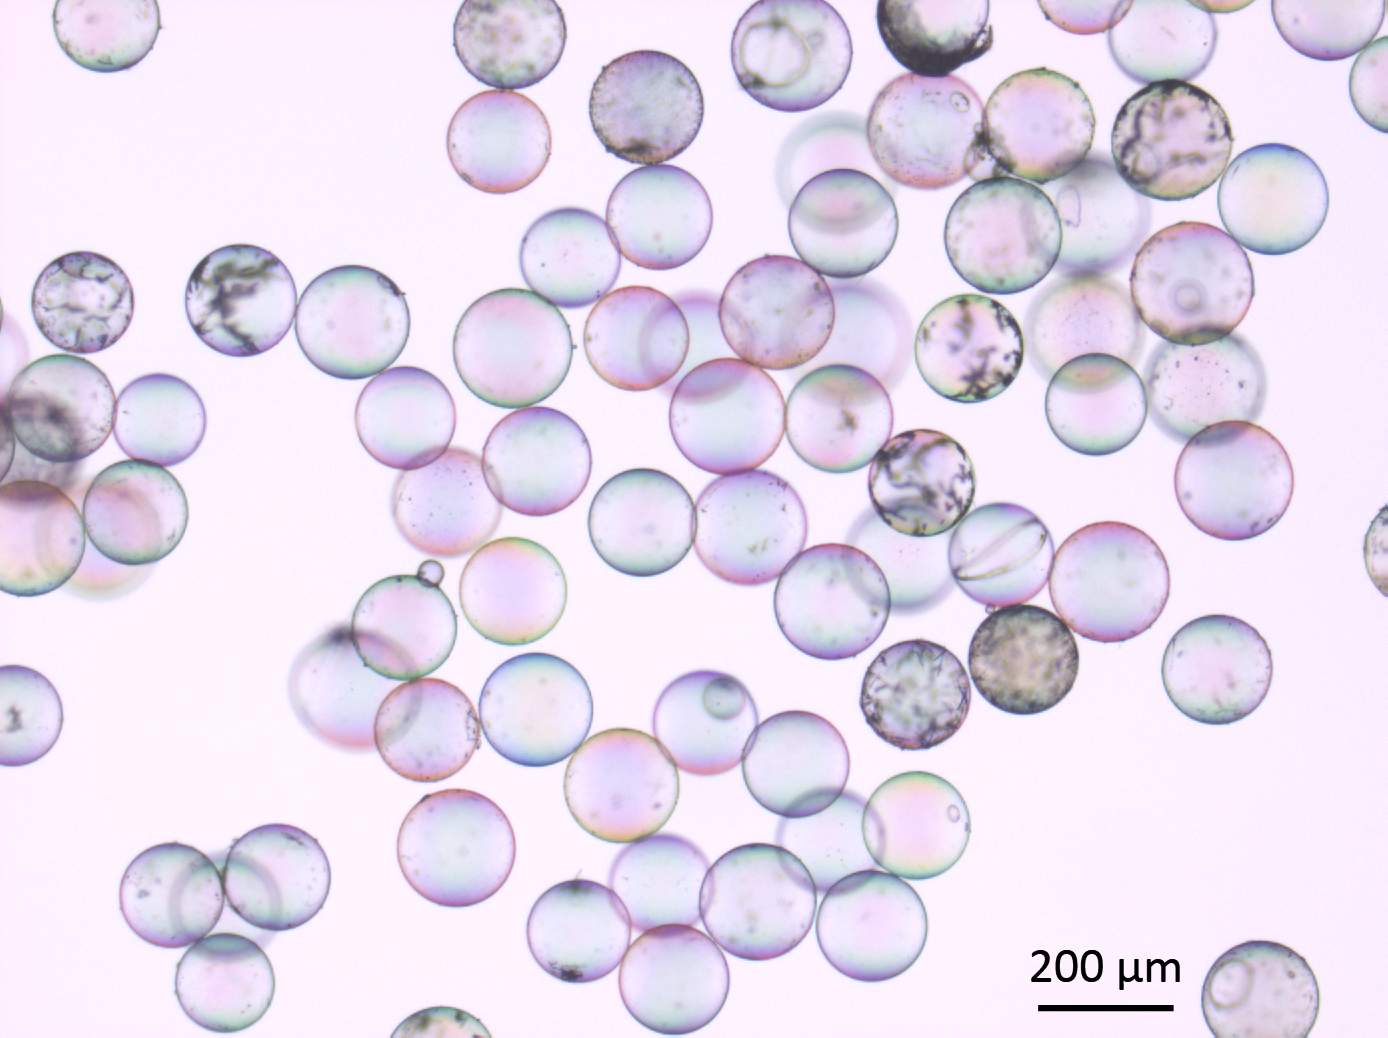
\includegraphics[width=\columnwidth]{hollow.png}
    \caption{\label{fig.hollow} Image of the hollow glass spheres used (Referenz
    oder am besten noch ein eigenes Mikroskopbild mit Massstab)}
\end{figure}

\begin{table}
\centering
\caption{Experimental parameters: Besides for the grain size, where the range is specified for all parameters deduced from this, only average values are given.}
\begin{tabular}{r|l}
Parameter&Value\\
\hline
particle size&165 $\rm \mu m$  $\pm$ 15 $\rm \mu m$\\
particle density&60 $\rm kg / m^3$ \\
inital particle number& 650\\
gas pressure&2100 Pa\\
initial dust-to-gas& 0.039 \\
final dust-to-gas& 0.018 \\
max. local dust-to-gas & 0.35 \\ 
friction time&7 ms\\
Knudsen number&0.08\\
rotation frequency& 0.336 Hz\\
Stokes number&0.0024\\
\label{para}
\end{tabular}
\end{table}

Observations were taken for 30s resulting in about 1 Million
particle positions.

\subsection{Dust-to-Gas ratios}

As dust-to-gas ratio $\epsilon$ we take the particle mass over gas mass within the volume initially filled with particles. 
Due to slow drifts and eventually due to collisions with the chamber walls, the particle
density decreases with time. This is shown in fig. \ref{fig.dtog}.

\begin{figure}[h]
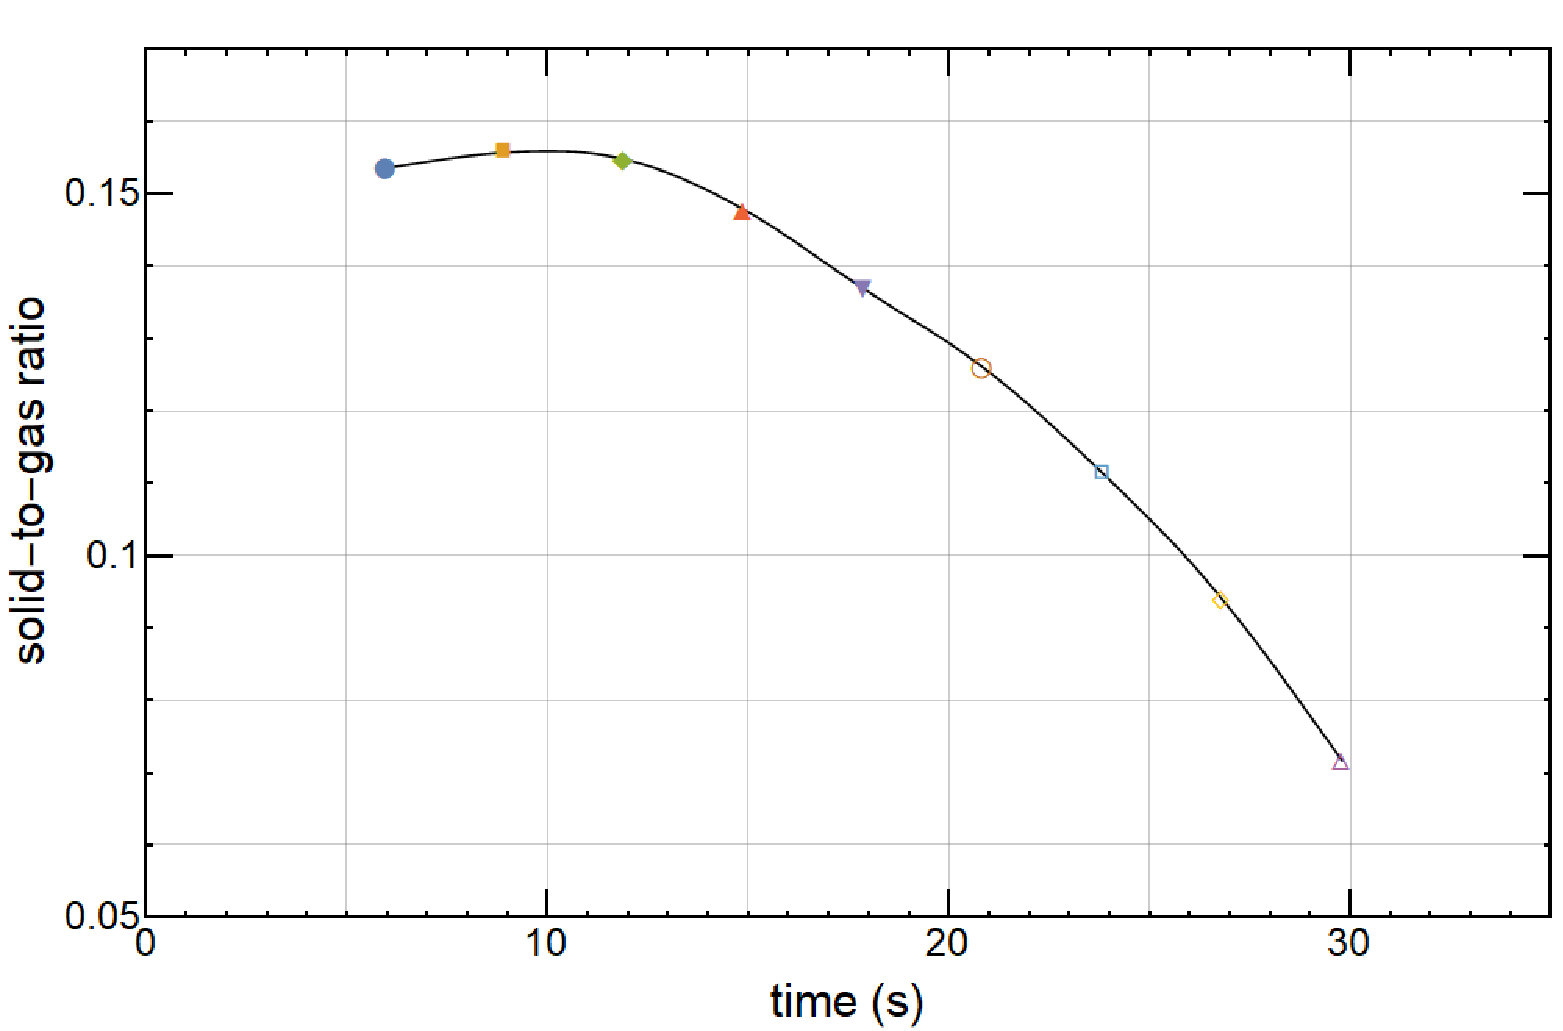
\includegraphics[width=\columnwidth]{density2.png}
    \caption{\label{fig.dtog}Average dust-to-gas ratio over time. Dust density is calculated with respect to injected particle depth.}
\end{figure}

It has to be noted that these values are calculated based on the average grain size, the observed number of grains and the thickness of the injected particle beam of 5 mm.
If the beam would disperse along the cylinder axis over time then the low densities at later times would be lower. 


\section{Grain Motion}

\subsection{Grain Motion at Low Particle Loading}

Especially at low dust-to-gas ratios the absolute gas coincide with the rigid rotation around the center with the set rotation frequency.
For all particles we calculate a relative velocity by assuming the gas to be in such a circular motion and subtracting this absolute motion.
Grains in steady state sedimentation should move on circular orbits in the laboratory 
reference frame with $v = \tau g$ relative to the gas then. Indeed this is the case. 

Fig. \ref{fig.circles} shows the motion of individual particles.
\begin{figure}[h]
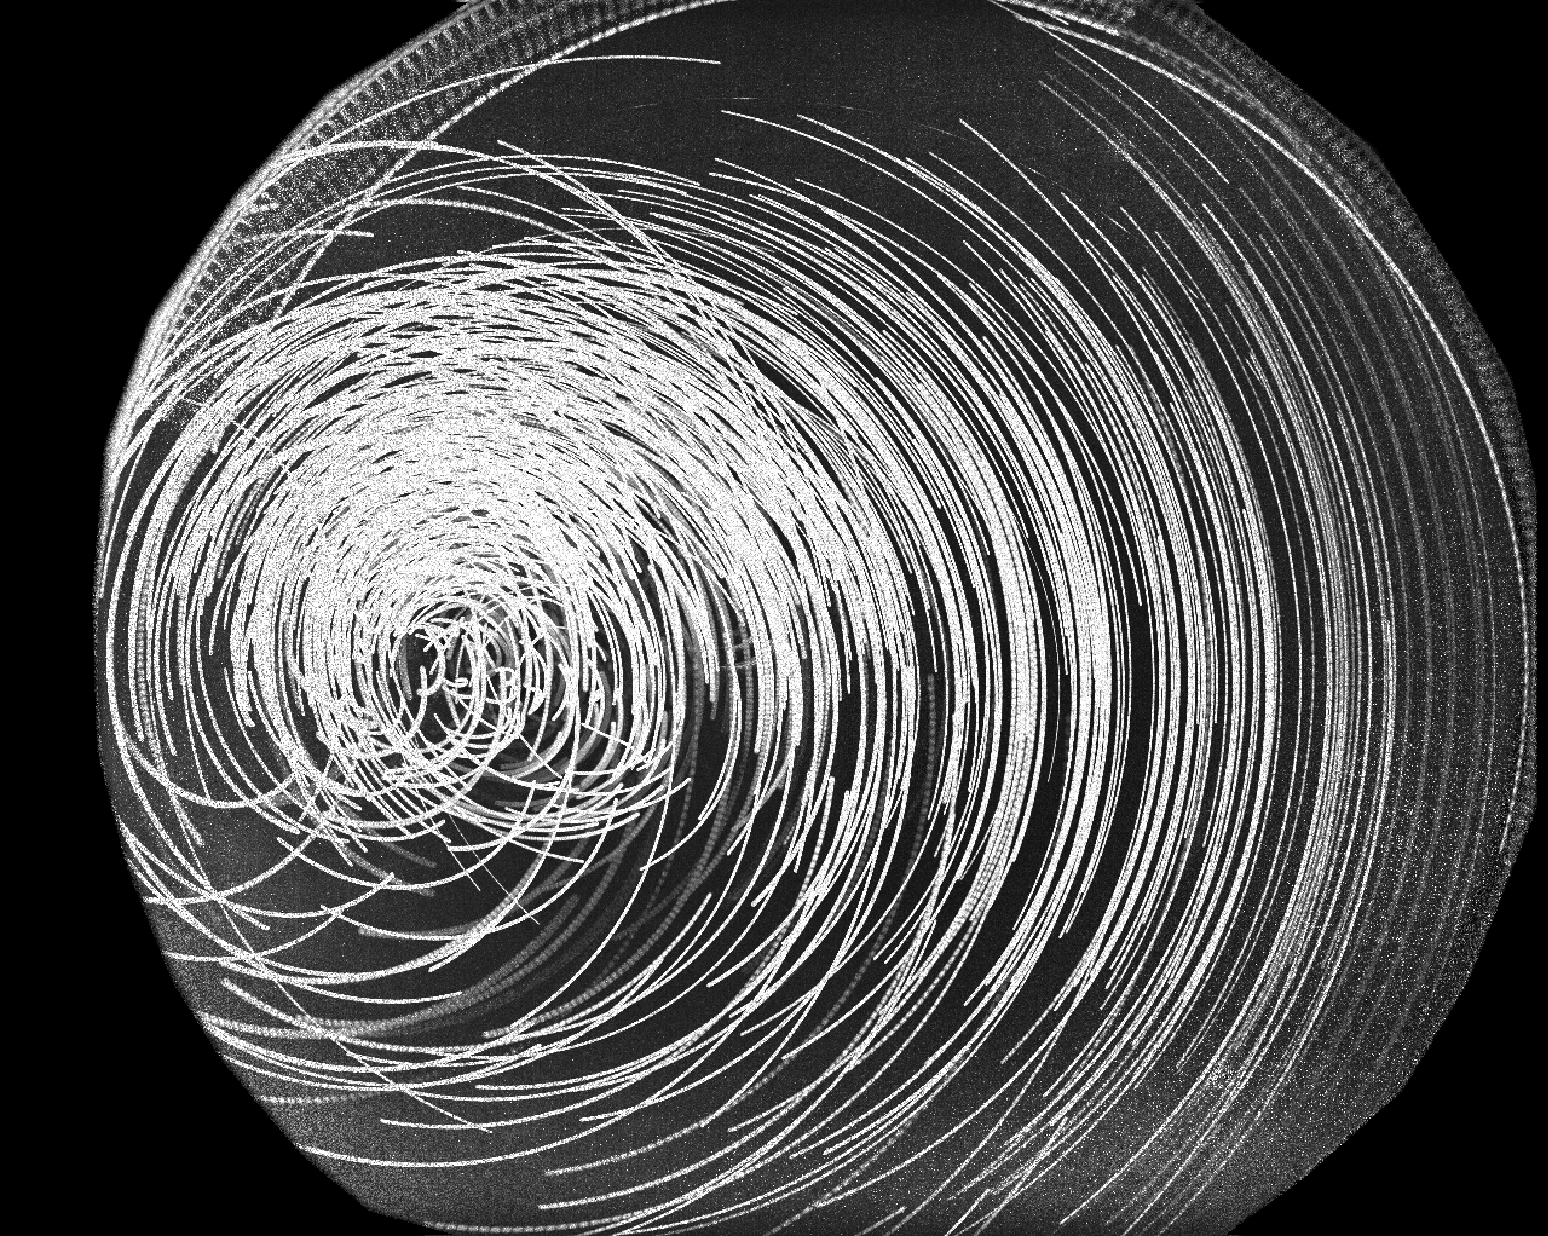
\includegraphics[width=\columnwidth]{round.png}
    \caption{\label{fig.circles} Circular particle tracks as superposition for part of a rotation. (noch einen Massstab einfuegen)}
\end{figure}
Due to the limited variation in particle size the point of stability which
is the center of the circles is similar for all particles.
The caculated sedimentation velocity for an average particle is 50 mm/s but this bears a number of uncertainties not well constrained. We therefore determined the sedimentation velocity of a single grain by dropping individual grains in a gas of the same pressure used here and find a sedimentation velocity of 69 mm/s, roughly consistent with the calculated value. This value for a single grain fits well with observed sedimentation velocities of the rotating grains at low particle loading with an average of 
67 mm/s (see fig. \ref{fig.vvonc} below). 
The closeness in this case reaches up to 20 /mm but has no influence on the average sedimentation velocity.

\subsection{Grain Motion at High Particle Loading}

While the average dust-to-gas ration only varies by about a factor of two between 
the beginning of the experimt (high ratio) and the end (low ratio) the influence on the particle motion is very strong.

Fig. \ref{fig.dtog2} shows a snapshot of the variations of local densities at early times with values up to $\epsilon \geq 0.3$.

\begin{figure}[h]
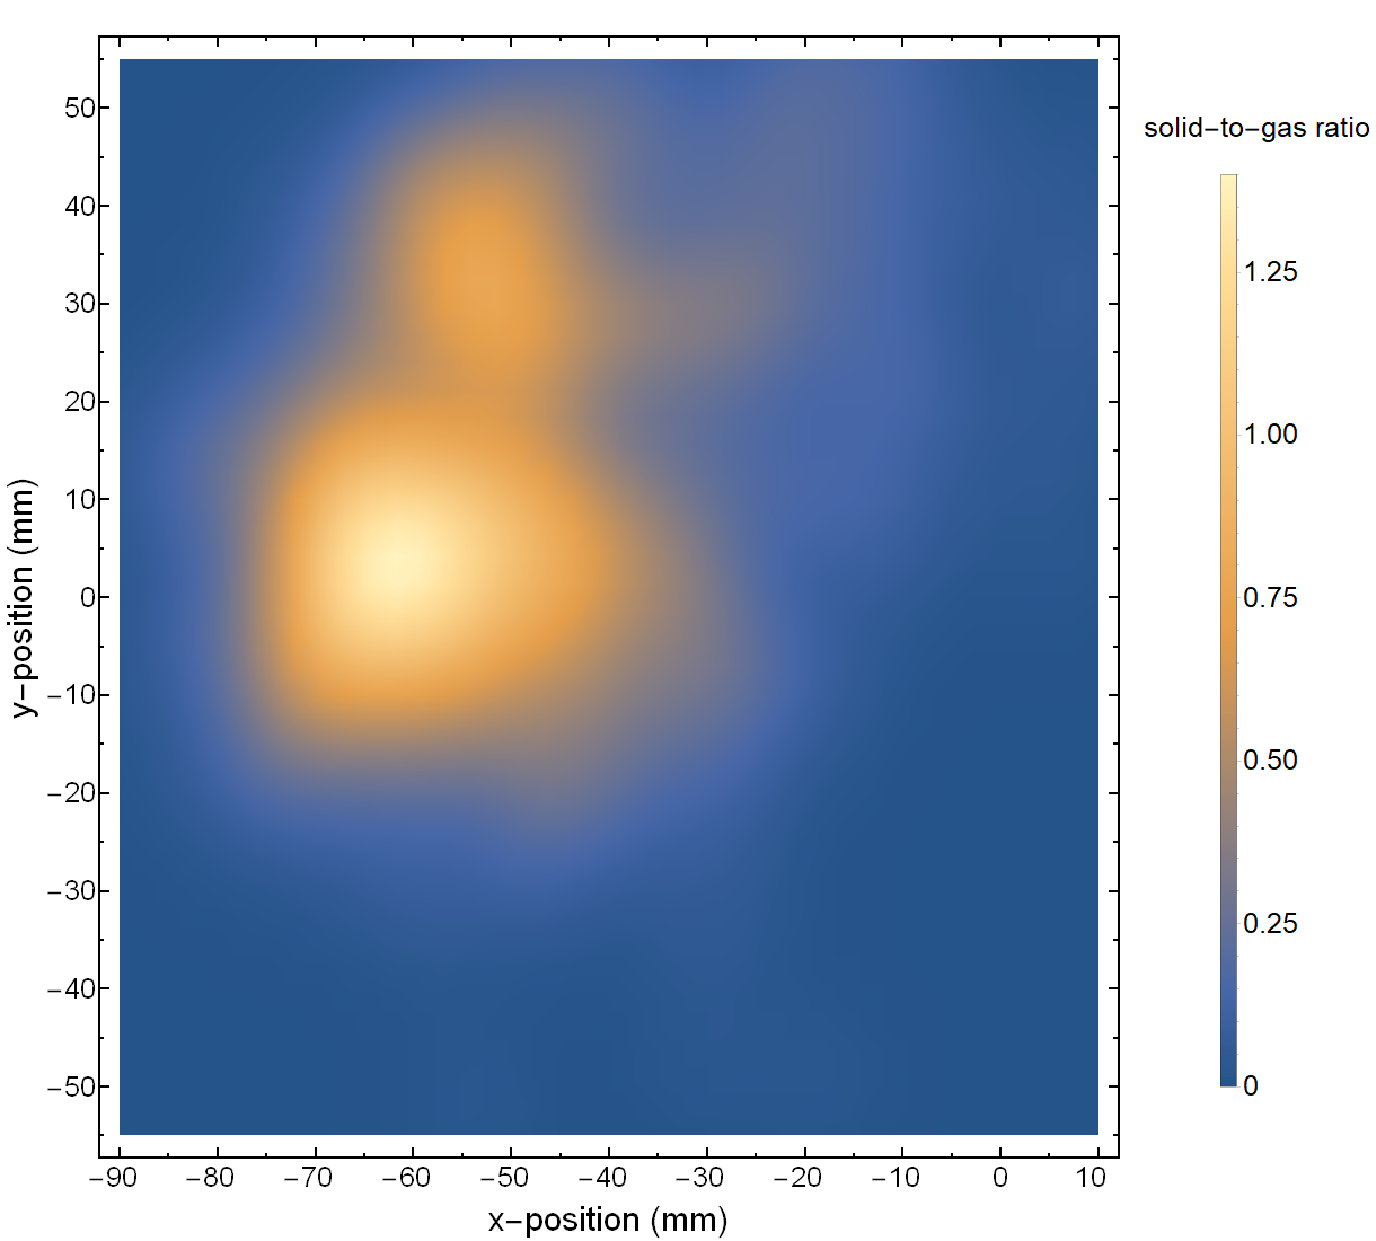
\includegraphics[width=\columnwidth]{density.png}
    \caption{\label{fig.dtog2}Snapshot of dust-to-gas ratio at early times (dense state)}
\end{figure}

Particles in regions with high closeness now sediment much faster than particles in less
close regions as seen in fig. \ref{fig.vvonc} (lower data). This figure shows the values averaged over full rotations of the experiment therefore increasing in time from xxx s 
(lower curve) to round 10 or xxx s (upper curve).

\begin{figure}[h]
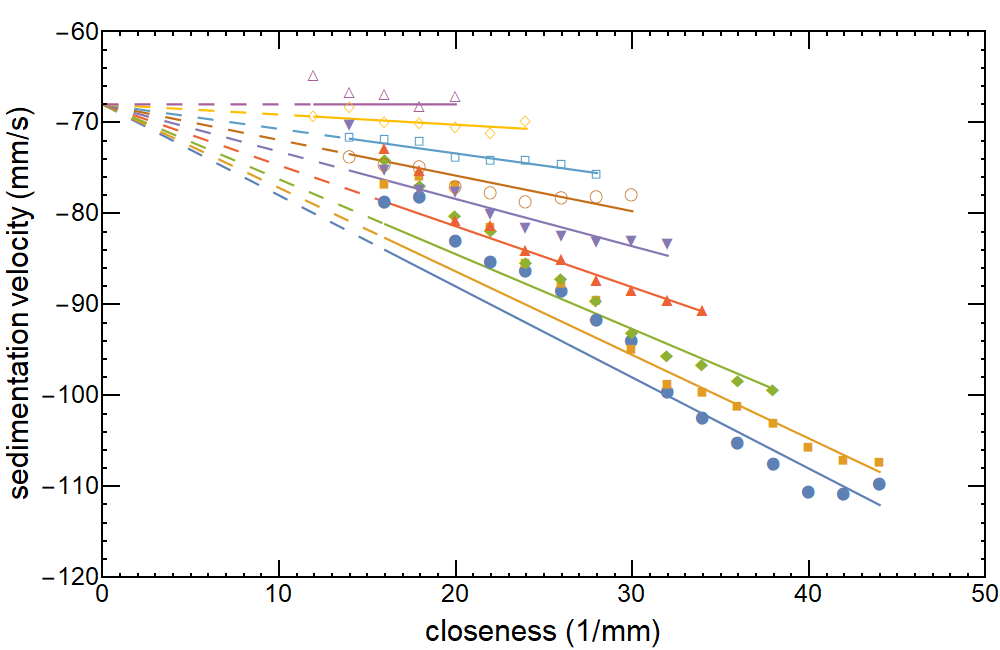
\includegraphics[width=\columnwidth]{vvonc.png}
    \caption{\label{fig.vvonc} Sedimentation velocity over closeness for individual rotations of the experiment. The evolution within the experiment chamber goes from initially dense (lower, 2nd round) to less dense (upper 10th round) cloud. Data are average values for typically xxx particles}
\end{figure}

As described above and visible in round 10 (fig. \ref{fig.vvonc}), particles at later, less dense times all sediment with the same speed also at a closeness 20 $\rm mm^{-1}$.
In contrast, in the high loading case also the speed of particles with small closeness 
increases with closeness. Obviously the system is more sensitive to closeness variations 
in this case. 

To a good first approximation the dependence of the sedimentation speed on closeness can be
described as linear or

\begin{equation}
v = v_0 - F_s \cdot C_i
\end{equation}

The sensitivity factor $F_s$ increases with the average of maximum closeness of the system or the dust-to-gas ratio as shown in fig. \ref{fig.sensitive1}.

\begin{figure}[h]
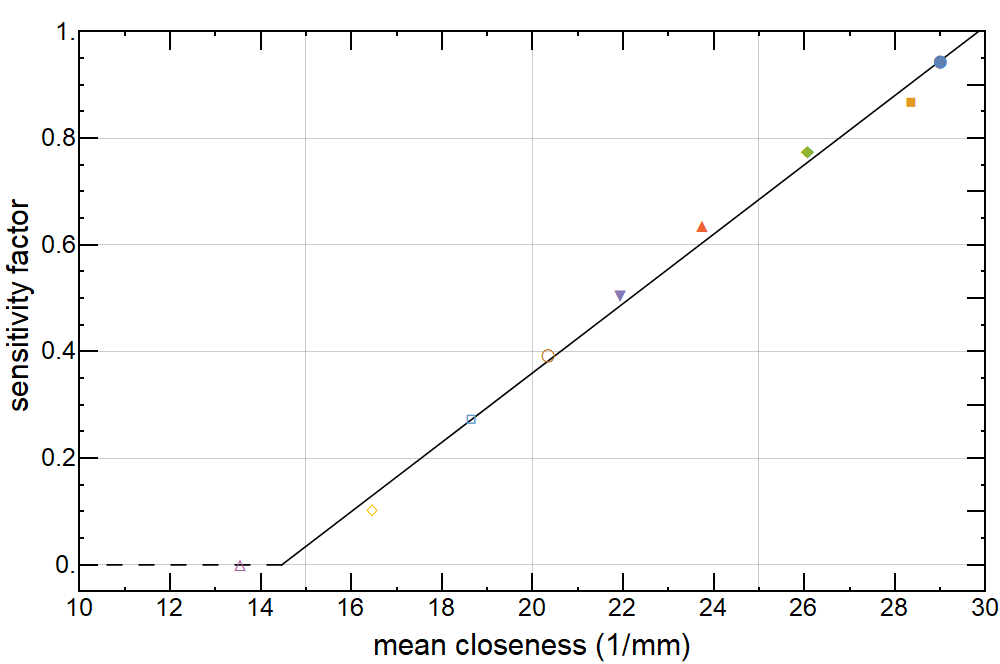
\includegraphics[width=\columnwidth]{sense1.png}
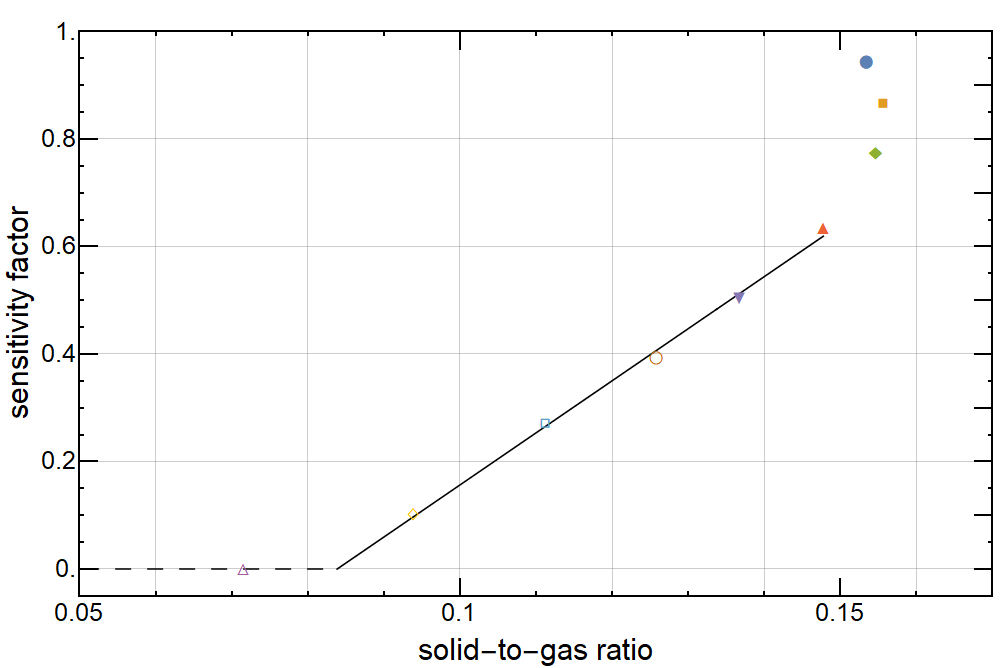
\includegraphics[width=\columnwidth]{sense2.png}
    \caption{\label{fig.sensitive1} Sensitivity factor dependence on average closeness (top) and dust-to-gas ratio (bottom)}
\end{figure}

A particle can enter a region of high closeness and sediment faster now. Nevertheless, a grain can also drop out of such a region. 
Trajectories of such particles are shown in fig. \ref{fig.entrain1}.

\begin{figure}[h]
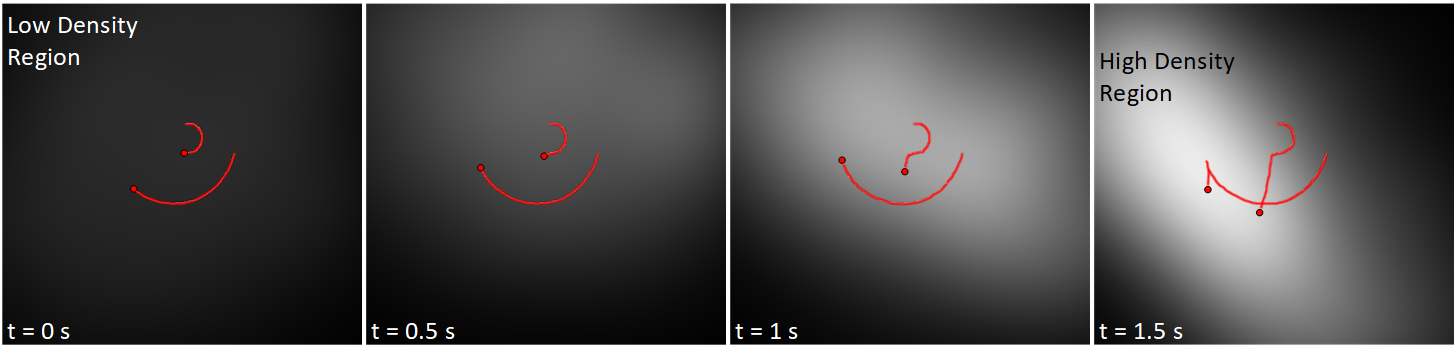
\includegraphics[width=\columnwidth]{track1.png}
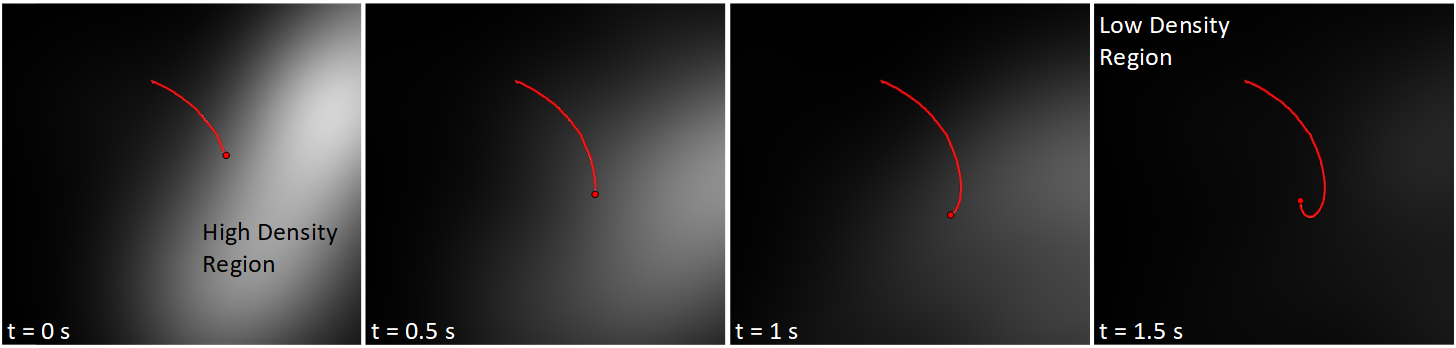
\includegraphics[width=\columnwidth]{track2.png}
    \caption{\label{fig.entrain1} top) particles entering a region of high closeness getting entrained and bottom) particle leaving a high closeness region staying behind}
\end{figure}

Fig. \ref{fig.track} shows the evolution of closeness attributed to a single particle over time
and the corresponding sedimentation speed.

\begin{figure}[h]
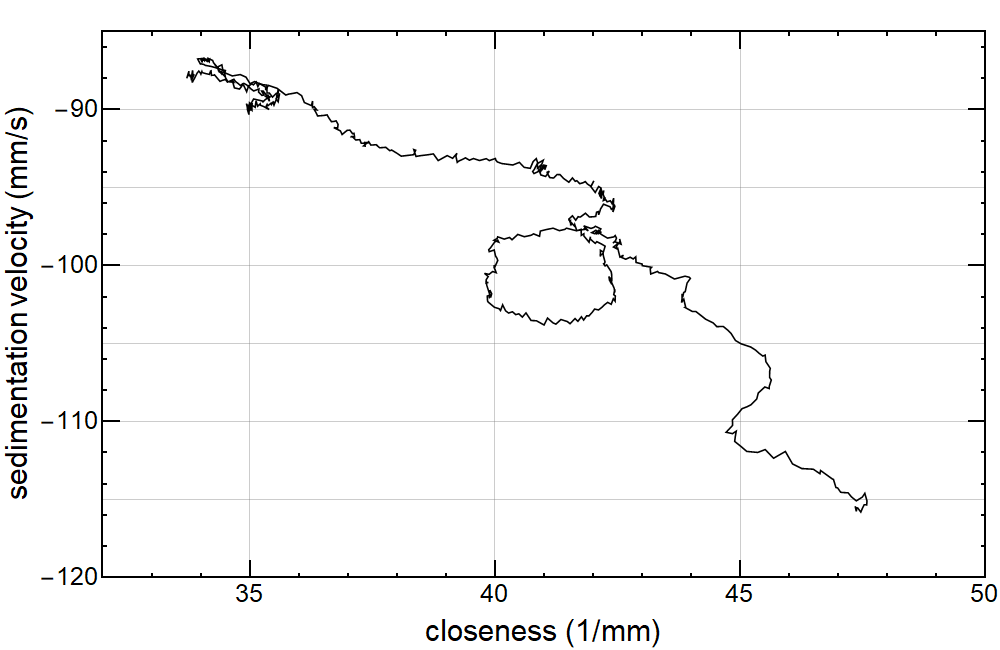
\includegraphics[width=\columnwidth]{track.png}
    \caption{\label{fig.track} Track of an individual particle within a closeness-velocity diagram.}
\end{figure}

At late times all particles on average sediment like individual grains with calculated sedimentation velocity. However, the speeds still vary due to variations in particle size. A typical velocity distribution (time xxx, round 9) is seen in fig. \ref{fig.speed1} (top).
At earlier times (time xxx, round 2) variations due to an increased sensitivity are added and the variations are much larger as seen in fig. \ref{fig.speed1} (bottom). 


\begin{figure}[h]
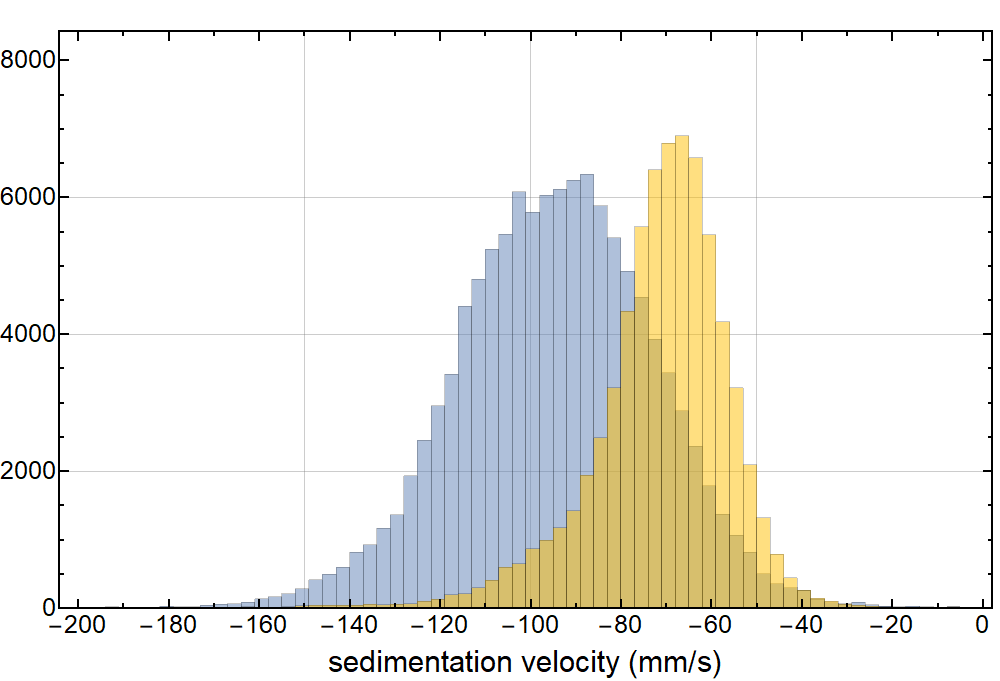
\includegraphics[width=\columnwidth]{veloc2and9.png}
    \caption{\label{fig.speed1} Sedimentation speed for low particle loading (right distribution) and high particle loading (left distribution)}
\end{figure}

Fig. \ref{fig.speed2} shows the closeness distribution changing from late to early.

\begin{figure}[h]
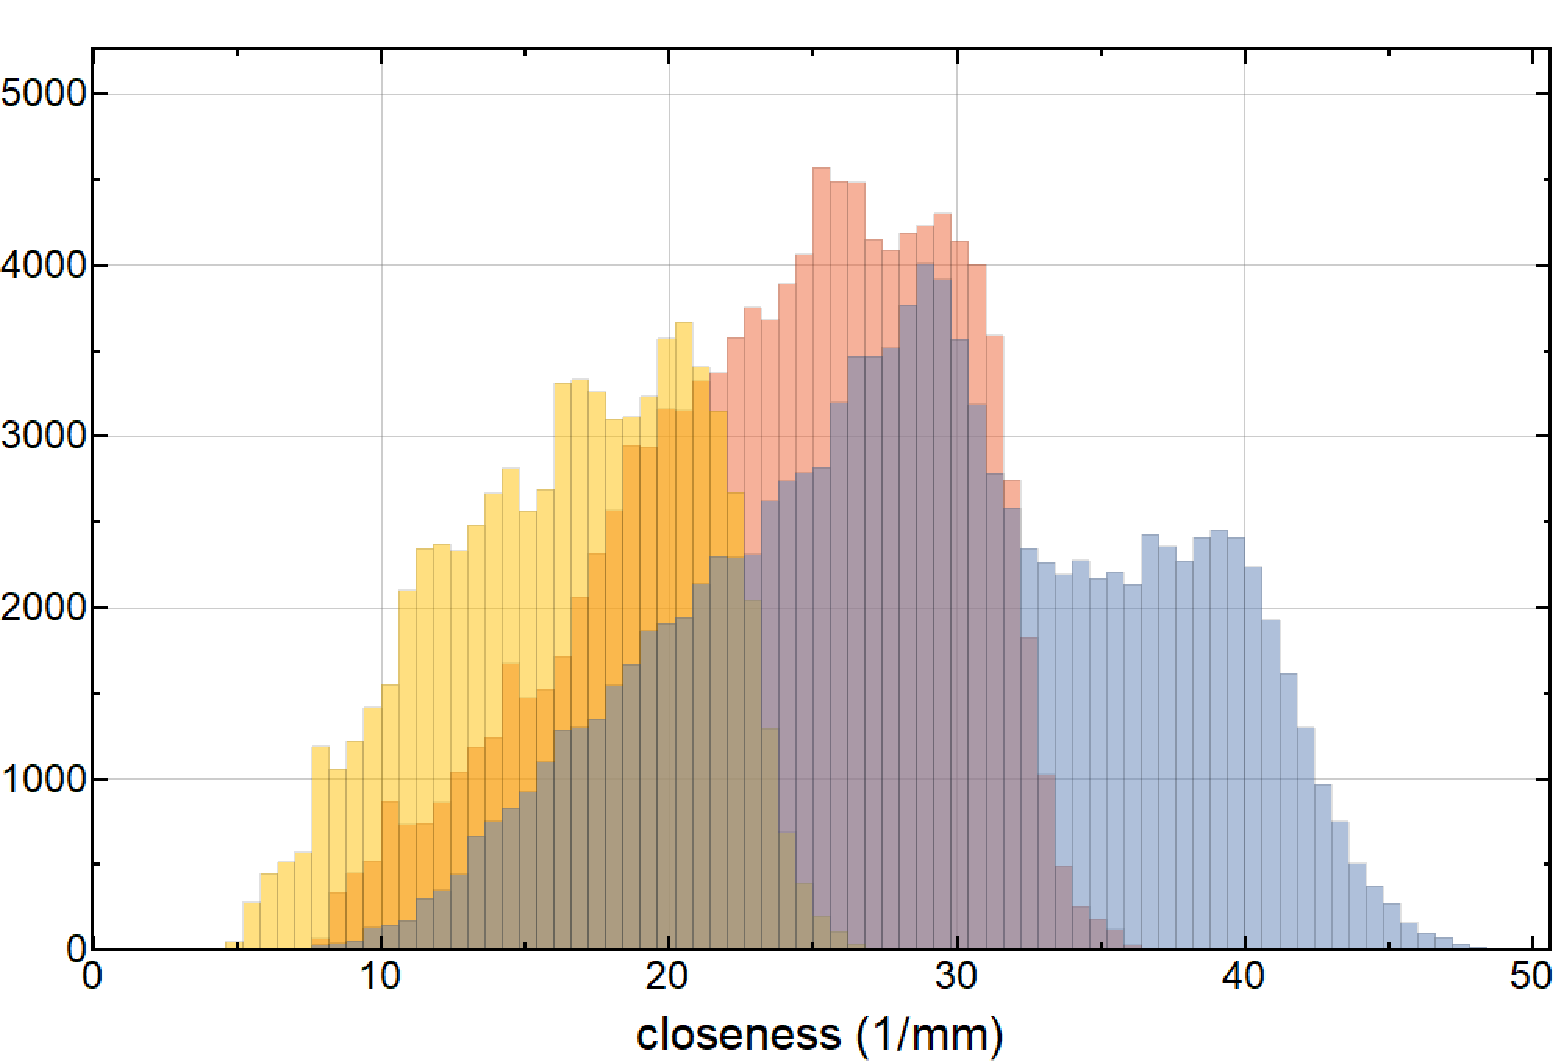
\includegraphics[width=\columnwidth]{close259.png}
    \caption{\label{fig.speed2} Evolution of the closeness distribution for 3 different times from rigth distribution (early) to left distribution (late)}
\end{figure}

As can be seen the initial closeness distribution has a wing at the high value side which it looses first. In general particle regions with high closeness get lost preferentially, leading to a inclined distribution with steeper drop off to higher values in general. 
This is due to the fact that particles sedimentating faster have a smaller stable region within the experiment to rotate and are easier lost to collisions with the wall.
Fig. \ref{fig.fluctuate} shows that the relative width in velocity essentially stays constant but the initial fluctuations at high dust-to-gas ratio are much broader.

\begin{figure}[h]
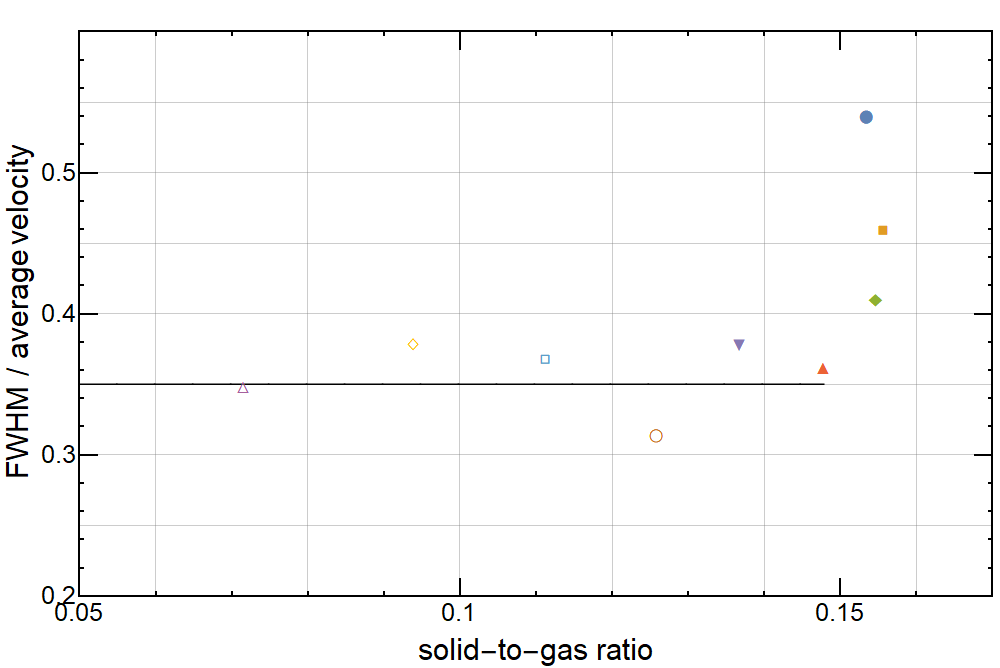
\includegraphics[width=\columnwidth]{fwhm_velocity.png}
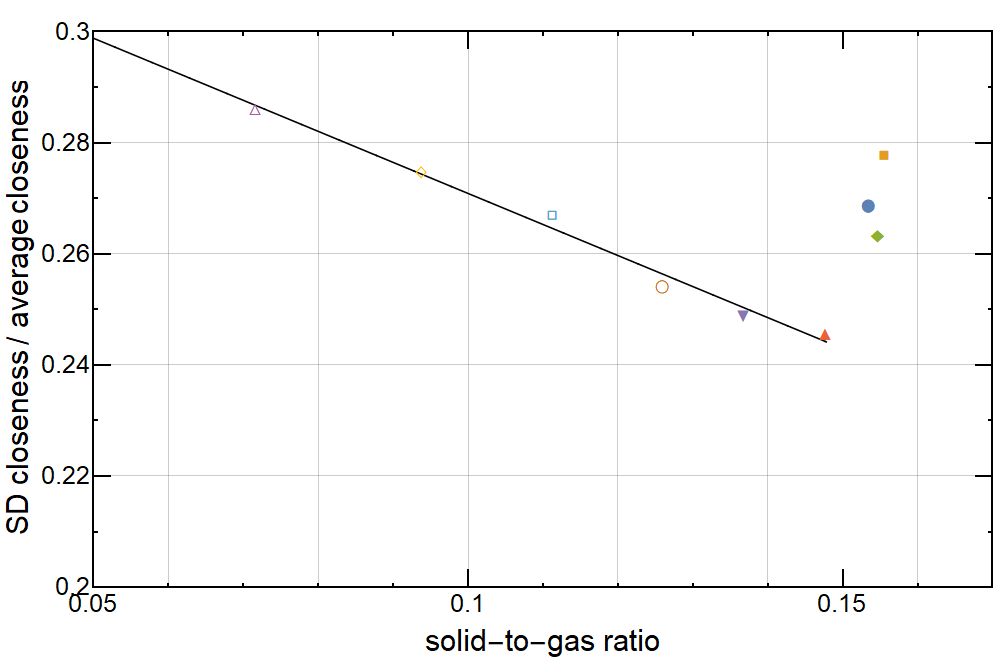
\includegraphics[width=\columnwidth]{sd_close.png}
    \caption{\label{fig.fluctuate} relative velocity width / average velocity and relative closeness width / average closeness over dust-to-gas ratio}
\end{figure}


\section{Discussion}


In this work we used the laboratory setup of a rotating experiment to study particle clouds at higher densities for a longer time in spite of sedimentation under Earth's gravity.
This allows an analysis of the particle motion in the presence of other particles for different conditions. 
Basic parameters are sedimentation velocity of individual particles and the average dust-to-gas ratio of the total particle cloud.
Variations in the \textit{local} dust-to-gas ratio are important but this value is not sufficient to describe the motion of a local particle cloud as it neglects the influence of neighboring regions on the particle motion. We therefore defined the closeness as another parameter
for each individual particle which depends on all particles and their distances 
to the particle considered.

We can separate two regimes of particle motion.
For dust-to-gas ratios below 0.02 particles behave like test particles embedded in a
gas. That means that they essentially do not feel the presence of the other particles or in other words they sediment like individual particles would sediment. There is no collective effect. This also holds for regions of varying closeness up to 20 $\rm mm^{-1}$. 

As closeness might not be an intuitive quantitiy, it might be argued that the largest closeness might still be representative for a dilute cloud corresponding to test particle behaviour. However, this argument does not hold for denser clouds.

For dust-to-gas ratios above 0.02 all particle motion does depend on closeness. So for
high dust loading also particles of closeness well below 20 $\rm mm^{-1}$ have much higher sedimentation speeds than individual grains as test particles should have. 
To first order the speed is now linear to closeness also for values of small closeness and the inclination of this linear dependence is sensitve to the dust-to-gas ratio or average closeness. 

We therefore defined the absolute of the inclination as sensitivity factor.
The sensitivity factor turns zero at a dust-to-gas ratio below 0.02 which quantifies the
separation of the two regimes of test particle behavior for lower values and collective
motion above.

For the high mass loading individual particles can change their motion by entering regions of high closeness, speeding up. However, they can also drop out again into
a region of lower closeness, slowing down. We do not see any concentration effect leading to a continuous local increase of particle density. This might be considered with care though as the experiment is biased to loosing sub-clouds of high closeness or particles with high sedimentation speeds. The stability point of fast particles is closer to the experiment wall and therefore the stability region is much smaller. Such regions are therefore preferentially lost due
to collisions with the walls. This is also visible in the evolution of the closeness distribution, where the large values decrease stronger than the small ones leading to
non-symmetric distribution with small slope rising but a steep slope falling off toward
larger closeness. In a way, the system cleans itself from 
very ''close'' or ''instable'' regions. 

The sensitivity factor shows that the average closeness might be better suited as description for the dense regime. At least 
the sensitivity factor is linear for all values of average closeness while there is a deviation from linearity for the highest dust-to-gas ratio. 

In the linear regime the absolute values of sedimentation velocities and the variation also varies, i.e. it gets broader for larger values or regions of higher closeness. So this certainly tends to include regions of larger speed. The change of width is linear to the average value as seen in the fact that the ratio of the width to average value is constant. Also here, the initially present overdense regions which are unstable in the experiment show stronger variations.

The closeness variations also depend on the absolute value of the average closeness.
The distribution gets slightly smaller with higher closeness but we would not give
this a fundamental interpretation in view of the experimental constrains on cloud stabilities.

Boiling this down, the essence of this work is the finding of increasing sensitivity
with increasing dust-to-gas ratio. For dilute systems a local increase in particle density -- or better in closeness -- has little effect. At high particle loading, small
changes lead to changes in sedimentation velocity of that region, the denser the more.
This implies that a self-amplification can work where denser regions move faster,
pick up grains and move still faster. So far we are only approaching this state as these
regions are unstable in the experiment being lost to the walls.
It is a strong indication though that streaming instabilities can also occur in laboratory
experiments.
\section{Summary}

To sum this up, for a given experiment we can describe the absolute value of the sedimentation velocity of a particle as 

\begin{equation}
v = v_0  \quad \texttt{for} \quad \epsilon < \epsilon_{crit}\\
\end{equation}
\begin{equation}
v = v_0 + \alpha \cdot (\epsilon-\epsilon_{crit}) \cdot C
\end{equation}

This might be compared to the simple assumption of a single particle clump of size $r_c$ sedimentating in an otherwise undisturbed gas.
\begin{equation}
v = v_0 + \beta \cdot (\epsilon - 0) \cdot r_c^2
\end{equation}

There are two principle differences. First, we do have a minimum solid to gas ratio, $\epsilon_{crit}$, for which collective motion gets important. Second, we traded the clump radius, $r_c$, for the closeness, $C$, as we do not have a well defined clump size
and closeness accounts for the local particle density as well as the distance between grains. 

\section{Caveats and Future Work}

There are limits in this work which might be improved in the future. 
Observations are only two dimensional and the particle distribution along the rotation axis is unknown. So absolute dust-to-gas ratios might probably systematically be estimated to high. This can be improved with an additional camera and viewing angle.
After many testing this work is essentially only based on the analysis of a single experiment (except the examples of particles entering and dropping out of dense region) as we had to develop an appropriate way of analysing dense many particle systems and to see where this might be going. Certainly, the database has to be extended but we
consider our work here as important milestone.

There might be interesting physics in the dense (high closeness) regions that 
are lost early on. Such regions might be kept longer if the coupling time of 
individual grains is be decreased. This is not easily achieved though as it 
requires smaller grains or grains of lower density which would be more prone
to aggregation adding complexity.

The Stokes number is still rather low. An increase is possible but requires faster rotations.
Also here, there experimental limits that still have to be explored in the future. 

It might be that it is exactly the regions of high closeness early on which are lost due to
instability in our experiment that correspond to instable regions in the sense of a streaming instability. This is only a speculation at this point though as it might be due to the initial conditions and did not evolve into this state on its own. Here, future experiments with low densitiy clouds which are compressed afterwards by some means will provide deeper insight.

We start with the premise at low particle loading that particles move 
through a gas in rigid rotation defining a relative sedimentation velocity. The gas motion will change in a more complex way in the case of high mass loadings. After all, it is the gas that mediates the coupling between grains. The calculated sedimentation velocity are therefore still a well defined construction but at some point
might loose the simple interpretation of relative velocity between grains and gas. 

To make the laboratory findings and laboratory extension more applicable to protoplanetary disks we intend to numerically simulate the experiment, gas and particles.

\section{Conclusion}

Johansen xxx studied the sensitivity of streaming depending on the metallicity in
protoplanetaryd disks. They find a strong dependenc varying
the solid-to-gas ratio from the standard 0.01 to only 0.04. While the setting is certainly very different in our experiments it is tantalizing that we also see a transition of particle motion at a particle loading of 0.02, which might be due to the general physics of 
particle-gas interaction. We see no collective behaviour for low dust-to-gas ratios up to 0.02. However, above this value all dust motion is getting increasingly sensitive to
small disturbances of the particle's closeness which eventually might end up in unstable situations. 
We define a Stokes number with respect to the experiment rotation timescale which turns out to be 0.002. This seems to be on the verge of triggering streaming instabilites (Yang,   xxx). 
Overall, our experiments support the ideas underlying streaming instabilities but also indicate that there is potential for future improvements which will hopefully lead us to well confirmed pictures of particle concentration and planetesimal formation by streaming instabilities.

\begin{acknowledgements}
This project is supported by DFG grant WU 321 / xxx and Kl xxx.
\end{acknowledgements}

% BibTeX users please use one of
%\bibliographystyle{spbasic}      % basic style, author-year citations
%\bibliographystyle{spmpsci}      % mathematics and physical sciences
%\bibliographystyle{spphys}       % APS-like style for physics
%\bibliography{}   % name your BibTeX data base

% Non-BibTeX users please use
\begin{thebibliography}{}
%
% and use \bibitem to create references. Consult the Instructions
% for authors for reference list style.
%
%\bibitem[De Beule et al. (2014)]{Beule} De Beule, C., Wurm, G., Kelling, T., K{\"u}pper, M., Jankowski, T., Teiser, J., The martian soil as a planetary gas pump, Nature Physics, 10, 17 (2014)


%\bibitem{RefJ}
% Format for Journal Reference
%Author, Article title, Journal, Volume, page numbers (year)
% Format for books
%\bibitem{RefB}
%Author, Book title, page numbers. Publisher, place (year)
% etc
\end{thebibliography}

\end{document}

